%----------------------------------------------------------------------------------------
%	PACKAGES AND THEMES
%----------------------------------------------------------------------------------------
\documentclass[aspectratio=169,xcolor=dvipsnames]{beamer}
\usetheme{SimplePlus}

\usepackage[brazilian]{babel}
\usepackage[utf8]{inputenc}
\usepackage{hyperref}
\usepackage{graphicx} % Allows including images
\usepackage{booktabs} % Allows the use of \toprule, \midrule and \bottomrule in tables
% \usepackage[table,dvipsnames]{xcolor}
\usepackage{tikz,tkz-base, tkz-fct,tikz-3dplot,tikz-cd,tkz-tab,tkz-euclide,pgf,pgfplots}
\usepackage{pstricks}
\usepackage{pst-plot}
\usepackage{systeme}
\usepackage{multicol}
\usepackage{lmodern,mathrsfs}
\usepackage{tasks}
\usepackage{float}
\usepackage{amsmath}
\usepackage{array}
\usepackage{multirow}
\usetikzlibrary{matrix} % LATEX and plain TEX

\pgfplotsset{compat=newest}

%----------------------------------------------------------------------------------------
%	TITLE PAGE
%----------------------------------------------------------------------------------------

\title[short title]{Análise Combinatória} % The short title appears at the bottom of every slide, the full title is only on the title page
% \subtitle{Subtitle}

\author[Fernando-Jorge] {Fernando Jorge}

\institute[NTU] % Your institution as it will appear on the bottom of every slide, may be shorthand to save space
{
  Escola Estadual Professor Lima Castro
}
\date{\today} % Date, can be changed to a custom date


%----------------------------------------------------------------------------------------
%	PRESENTATION SLIDES
%----------------------------------------------------------------------------------------

\begin{document}

\begin{frame}
    % Print the title page as the first slide
    \titlepage
\end{frame}

\begin{frame}{Sumário}
    % Throughout your presentation, if you choose to use \section{} and \subsection{} commands, these will automatically be printed on this slide as an overview of your presentation
    \tableofcontents
\end{frame}

%------------------------------------------------
\section{Princípio Fundamental da Contagem}
%------------------------------------------------

\begin{frame}{O que é análise combinatória?}
A análise combinatória é um ramo da matemática que procura elaborar métodos que nos permitam encontrar o número de possibilidades que um evento pode ocorrer, sem a obrigatoriedade de descrevermos todos os eventos possíveis.

 É importante conhecermos tais métodos, pois nem sempre temos condições de descrever todas as formas sob as quais uma situação pode ocorrer, principalmente em situações onde a resposta é um número muito elevado.

\end{frame}

%------------------------------------------------

\begin{frame}{Princípio Fundamental da Contagem}
    Se um experimento \textit{E} pode apresentar \textit{n} resultados distintos e um experimento \textit{F} pode
    apresentar \textit{k} resultados distintos, então o número de resultados distintos que o experimento composto
    de \textit{E} e \textit{F} pode apresentar, nessa ordem, é dado pelo produto $n \cdot k$
\end{frame}

%------------------------------------------------

\begin{frame}{Princípio Fundamental da Contagem}
    João foi convidado para festa de sua amiga Maria. Muito vaidoso, abriu o seu guarda-roupa e experimentou todas as roupas que possuía:  3 camisetas e 2 bermudas.
      \begin{figure}[htb!]
        \centering
        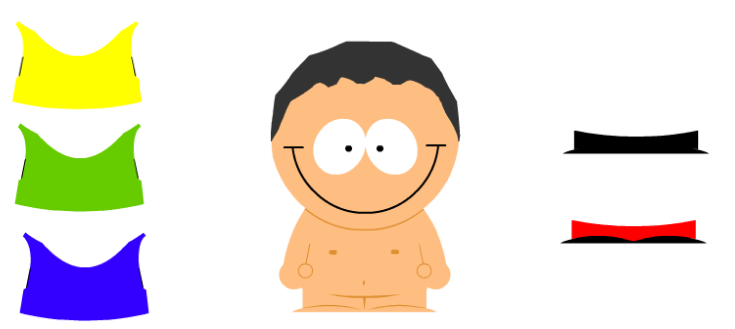
\includegraphics[width=.5\linewidth]{images/im1.png}
      \end{figure}
    De quantas formas João pode se arrumar?

\end{frame}

%------------------------------------------------

\begin{frame}[t]{Princípio Fundamental da Contagem}
    Um restaurante oferece no cardápio 2 entradas distintas, 3 tipos de pratos principais e 3 sobremesas diferentes.
    Uma pessoa deseja uma salada, um prato principal e uma sobremesa. De quantas maneiras a pessoa
    poderá fazer seu pedido?
\end{frame}


%------------------------------------------------

\begin{frame}[t]{Princípio Fundamental da Contagem}
    \begin{center}
        Cuidado com o uso do PFC para eventos dependentes!
    \end{center}
    O diretor de uma empresa precisa escolher para o setor de compras um coordenador e um vice dentre 5 funcionários (A, B, C, D, E) . De quantas formas pode se dar essa escolha?
\end{frame}

%------------------------------------------------

\section{Fatorial}

\begin{frame}{Fatorial}
    Sendo \textit{n} um número natural, define-se fatorial de \textit{n}, e indica-se:
    \begin{equation*}
        n! = n \cdot (n -1) \cdot (n-2) \cdot \dots \cdot 3 \cdot 2 \cdot 1
    \end{equation*}

    \begin{itemize}
        \item $0! = 1$
        \item $1! = 1$
        \item $2! = 2 \cdot 1 = 2$
        \item $3! = 3 \cdot 2 \cdot 1 = 6$ \\ \hspace{1cm} \vdots
        \item $n! = n \cdot (n -1) \cdot (n - 2) \cdot \dots \cdot 3 \cdot 2 \cdot 1$
    \end{itemize}

\end{frame}

%------------------------------------------------

\begin{frame}{Fatorial}
    Podemos escrever os fatoriais em função de fatoriais menores:

    \begin{itemize}
        \item $5! = 5 \cdot 4!$
        \item $5! = 5 \cdot 4 \cdot 3!$
        \item $5! = 5 \cdot 4 \cdot 3 \cdot  2!$
    \end{itemize}
\end{frame}

%------------------------------------------------

\begin{frame}{Fatorial}
    \begin{center}
        Veja os exemplos
    \end{center}

    \begin{itemize}
        \setlength\itemsep{1em}
        \item $\dfrac{10!}{8!}$
        \item $\dfrac{50! - 49!}{49!}$
        \item $\dfrac{(n+1)!}{(n-1)!} = 210$
    \end{itemize}

\end{frame}

%------------------------------------------------
\section{Tipos de Agrupamento}

\begin{frame}{Tipos de Agrupamento}
    Um agrupamento de elementos é qualquer conjunto, ordenado ou não, formados por esses elementos. São classificados dois tipos fundamentais de agrupamentos: ARRANJO e COMBINAÇÃO.
\end{frame}

\begin{frame}{Arranjo}
    ARRANJOS são Agrupamentos em que se \textit{considera a ordem dos elementos}, ou seja, resultados com mesmos
    elementos mas em ordens diferentes são considerados distintos. Veja a seguinte situação:
    \vspace{.5cm}

    ``O professor de Matemática precisa escolher 3 alunos dentre 10 para participarem de uma comissão ocupando os cargos de presidente, vice-presidente e secretário''
    \vspace{.5cm}

    Considere a notação (Presidente, Vice-presidente, Secretário)
    \vspace{.5cm}

    \textbf{Note que o resultado (A1, A2, A3) é diferente do resultado (A2, A1, A3).}

\end{frame}

\begin{frame}{COMBINAÇÃO}
    COMBINAÇÕES são agrupamentos em que NÃO se considera a ordem dos elementos, ou seja, resultados com mesmos elementos, ainda que em ordens diferentes, são considerados iguais. Veja a seguinte situação:

    \vspace{.5cm}
    ``O professor de Matemática precisa escolher 3 alunos dentre 10 para participarem de uma visita técnica''.
    \vspace{.5cm}

    \textbf{Note que o resultado (A1, A2, A3) é igual ao resultado (A2, A1, A3).}
\end{frame}

\section{Permutação}
\begin{frame}{Permutação Simples}
    Uma permutação simples dos elementos de um conjunto F é qualquer sequência de elementos distintos formado por todos os elementos de F. A permutação é um caso específico de Arranjo. Veja a situação:
    \vspace{.5cm}

    ``De quantas maneiras pode-se organizar 6 livros distintos em uma prateleira?''
    \vspace{.5cm}

    Pelo PFC, temos: $6 \cdot 5 \cdot 4 \cdot 3 \cdot 2 \cdot 1 = 720$ maneiras
    \vspace{.5cm}

    Generalização:

    Permutação Simples de \textit{n} elementos: $P_n = n!$

\end{frame}

\begin{frame}[t]{Permutação Simples}
    De quantas formas podem 5 pessoas ficar em fila indiana?
\end{frame}

\begin{frame}[t]{Permutação Simples}
    Quantas palavras distintas podemos formar com a palavra PERNAMBUCO? Quantas começam com a síIaba PER?
\end{frame}

\begin{frame}[t]{Permutação com Elementos Repetidos}
    De quantas maneiras pode-se organizar 6 livros em uma prateleira sendo que 3 deles são iguais?
      \begin{figure}[htb!]
        \centering
        
\includegraphics[width=.3\linewidth]{images/im3.png}
      \end{figure}
\end{frame}

\begin{frame}{Permutação com Elementos Repetidos}
    Fórmula:

    \begin{equation*}
        P_n^{k_1, k_2, k_3, \dots , k_p} = \dfrac{n!}{k_1!k_2!k_3!\dots k_p!}
    \end{equation*}
\end{frame}

\begin{frame}{Permutação Circular}
    De quantas maneiras podemos dispor quatro pessoas ao redor de uma mesa circular?

    \begin{figure}[htb!]
      \centering
        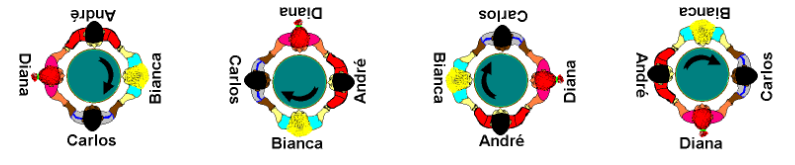
\includegraphics[width=.8\linewidth]{images/im4.png}
    \end{figure}

\end{frame}

\begin{frame}{Permutação Circular}
    Fórmula:

    \begin{equation*}
    P_{c(n)} = \dfrac{n!}{n}
    \end{equation*}

\end{frame}

\begin{frame}{Arranjo}
    Como já vimos anteriormente, arranjos são agrupamentos em que se \textbf{considera a ordem dos elementos}.
    \vspace{.5cm}

    Muito comum em questões de criação de senhas, números, telefones, placas de carro, competições, disputas, situações em que houver hierarquia.

    \vspace{.5cm}

    Fórmula:

    \begin{equation*}
        A_p^n = A_{n,p} = \dfrac{n!}{(n-p)!}
    \end{equation*}

    \vspace{.5cm}

    Dica: Questões de Arranjos podem ser resolvidos utilizando PFC.

\end{frame}

\begin{frame}[t]{Arranjo}
    Veja algunas exemplos:

    \vspace{.5cm}

    \begin{itemize}
        \setlength\itemsep{1em}
        \item $A_{5,2} = $
        \item $A_{10,4} = $
        \item $A_{8,1} = $
        \item $A_{7,5} = $
    \end{itemize}

\end{frame}

\begin{frame}[t]{Arranjo}
    Um cofre possui um disco marcado com os dígitos 0, 1, 2, ..., 9. O segredo do cofre é marcado
por uma sequência de 3 dígitos distintos. Se uma pessoa tentar abrir o cofre, quantas tentativas
deverá fazer (no máximo) para conseguir abri-lo?
\end{frame}

\begin{frame}[t]{Arranjo}
    Em uma escola está sendo realizado um torneio de futebol de salão, no qual dez times estão
participando. Quantos jogos podem ser realizados entre os times participantes em turno e
returno?
\end{frame}

\begin{frame}{Combinação}
    Como já vimos anteriormente, combinações são agrupamentos em que \textbf{não considera-se a ordem dos elementos}.

    \vspace{.5cm}

    Muito comum em questões de criação de grupos, comissões e agrupamentos em que não há distinção pela ordem dos elementos escolhidos.

    \vspace{.5cm}

    Fórmula:

    \begin{equation*}
        C_p^n = C_{n,p} = \dfrac{n!}{(n-p)!p!}
    \end{equation*}

    \vspace{.5cm}

    Dica: Questões de Combinações não podem ser resolvidos utilizando PFC.
\end{frame}

\begin{frame}[t]{Combinação}
    Veja alguns exemplos:

    \vspace{.5cm}

    \begin{itemize}
        \setlength\itemsep{1em}
        \item $C_{5,2} = $
        \item $C_{10,4} = $
        \item $C_{8,1} = $
        \item $C_{7,5} = $
    \end{itemize}

\end{frame}

\begin{frame}[t]{Combinação}
    Uma prova consta de 5 questões das quais o aluno deve resolver 2. De quantas formas
    ele poderá escolher as 2 questões?
\end{frame}

\begin{frame}[t]{Combinação}
    Os 32 times que jogarão a Copa do Mundo 2014 no Brasil estão agrupados em oito grupos de
quatro seleções cada. As quatro seleções de cada grupo se enfrentarão uma única vez entre si,
formando a primeira etapa da copa. Calcule a quantidade de jogos que cada grupo terá.
\end{frame}

\end{document}
